\section{Grundlagen und Definitionen}
In diesem Abschnitt geht es um die Definitionen und Namenskonventionen, die für Operatorpräzedenzsprachen (OPL) benötigt werden. Zunächst kommt eine kurze Definition von kontextfreien Grammatiken, gefolgt von Definitionen und Einschränkungen für Operatorpräzedenzgrammatiken (OPG). Im Anschluss wird die Klasse der Operatorpräzedenzautomaten (OPA) eingeführt, sowohl deterministisch als auch nichtdeterministisch, sowie deren Äquivalenz zu OPGs bewiesen. Die Definitionen richten sich nach \cite{precedence_automata} \cite{mso} und \cite{op_vpl_property}.
\subsection{Operatorpräzedenzgrammatik}
Eine kontextfreie Grammatik (kfG) ist ein 4-tupel $G = (N, \Sigma, P, S)$, wobei N die Menge der Nichtterminalsymbole, $\Sigma$ die Menge der Terminalsymbole, P die Menge der Produktionsregeln und S das Startsymbol bezeichnet. Folgende Namenskonventionen werden im weiteren Verlauf verwendet: Kleine lateinische Buchstaben am Anfang des Alphabets $a, b, ...$ bezeichnen einzelne Terminalsymbole; spätere, kleine lateinische Buchstaben $u,v, ...$ bezeichnen Terminalstrings; große lateinische Buchstaben $A, B, ...$ stehen für Nichtterminalsymbole und griechische Buchstaben $\alpha, \beta, ...$ für beliebige Strings über $N \cup \Sigma$. Wenn $S \overset{*}{\Rightarrow} \alpha$, nennt man $\alpha$ eine \textit{Satzform}. Sofern nicht explizit eingeschränkt können Strings auch leer sein.\\
Weiterhin haben Produktionsregeln die Form $A \rightarrow \alpha$ mit der \textit{leeren Regel} $A \rightarrow \epsilon$. \textit{Umbenennende} Regeln haben nur ein Nichtterminalsymbol als rechte Seite . Eine \textit{direkte Ableitung} wird mit $\Rightarrow$ beschrieben, eine beliebige Anzahl von Ableitungen mit $\overset{*}{\Rightarrow}$. 
\\
Eine Grammatik heißt \textit{reduziert}, wenn jede Regel aus P benutzt werden kann um einen String aus $\Sigma\textsuperscript{*}$ zu erzeugen. Sie ist \textit{invertierbar}, wenn keine zwei Regeln identische rechten Seiten haben. Für eine kfG G kann eine \textit{geklammerte Grammatik} $\tilde{G}$ erstellt werden, in der jede rechte Regelseite mit Klammersymbolen $[,] \notin \Sigma$ umgeben ist. Zwei Grammatiken $G$ und $G^\prime$ sind \textit{äquivalent}, wenn sie die gleiche Sprache generieren, $L(G)=L(G^\prime)$. Wenn zusätzlich gilt $L(\tilde{G})=L(\tilde{G^\prime})$ sind sie auch \textit{strukturell äquivalent}.\\

Eine Regel ist in \textit{Operatorform}, wenn ihre rechte Seite keine benachbarten Nichtterminale hat. Entsprechend heißt eine Grammatik, die nur solche Regeln beinhaltet, \textit{Operatorgrammatik} (OG). Jede kfG $G=(N,\Sigma, P, S)$ kann in eine äquivalente Operatorgrammatik $G'=(N', \Sigma, P', S)$ umgewandelt werden \cite{og, salomaa1973formal}. Die folgenden Definitionen gelten für Operatorpräzedenzgrammatiken (OPGs). \\
\begin{definition}

Für eine OG G und ein Nichtterminal A sind die \textit{linken und rechten Terminalmengen}  definiert als 
$$ \mathcal{L} \textsubscript{G}(A) = \{ a \in \Sigma | A \overset{*}{\Rightarrow} Ba \alpha \}, \;
 \mathcal{R} \textsubscript{G}(A) = \{ a \in \Sigma | A \overset{*}{\Rightarrow} \alpha aB \}$$
mit $B \in N \cup \{\epsilon\}$
\end{definition}

Der Name G der Grammatik wird ausgelassen, sofern der Kontext klar ist. Eines der wichtigsten Merkmale von Operatorpräzedenzgrammatiken ist die Definition von drei binären Operatorpräzedenzrelationen.
\begin{definition}[Präzedenzrelationen]\ \\
\label{relationen}
Gleiche Präzedenz: $ a \doteq b \Leftrightarrow \exists A \rightarrow \alpha aBb \beta , 
		B \in N \cup \{ \epsilon \}$ \\
		Übernimmt Präzedenz: $ a \gtrdot b \Leftrightarrow \exists A \rightarrow \alpha Db \beta , D \in N $ and $ a \in
		\mathcal{R}\textsubscript{G}(D)$ \\
		Gibt Präzedenz ab: $ a \lessdot b \Leftrightarrow \exists A \rightarrow \alpha aD \beta , D \in N $ and $ b \in
		\mathcal{L}\textsubscript{G}(D)$
\end{definition}
Es muss beachtet werden, dass diese Relationen im Gegensatz zu ähnlichen arithmetischen Relationen (<,>,=) keine transitiven, symmetrischen oder reflexiven Eigenschaften aufweisen. Weiterhin schließt die Gültigkeit einer Relation die andere nicht aus, sodass z.B. sowohl $a \lessdot b$ als auch $a \doteq b$ gelten kann.
Für eine OG G kann eine Operatorpräzedenzmatrix (OPM) $M = OPM(G)$ als $|\Sigma | \times |\Sigma |$ erstellt werden, die für jedes geordnete Paar $(a,b)$ die Menge $M \textsubscript{ab}$ der Operatorpräzedenzrelationen beinhaltet. Für solche Matrizen sind Inklusion und Vereinigung natürlich definiert.

\begin{definition}
Eine OG G ist eine OPG oder auch Floyd Grammatik gdw. M = OPM(G) eine \textit{konfliktfreie} Matrix ist.\\ 
Also: $\forall a, b, |M \textsubscript{ab} | \leq 1$\\
Eine OPL ist eine Sprache, die durch eine OPG gebildet wird.
\end{definition}

Für solche OPMs werden nun weitere Namenskonventionen vereinbart. Zwei Matrizen sind \textit{kompatibel}, wenn ihre Vereinigung konfliktfrei ist. Eine Matrix heißt \textit{total}, wenn gilt $\forall a, b: M \textsubscript{ab} \neq \emptyset$. Für eine OPM M ist die Klasse der präzedenzkompatiblen OPGs als $C_M=\{G \in OPG | OPM(G) \subseteq M\}$ definiert. 
Für eine OPG wird die \textit{Fischer Normalform (FNF)} definiert.

\begin{definition}[Fischernormalform]
Eine OPG G ist in Fischer Normalform gdw. gilt:
\begin{itemize}
\item
G ist invertierbar,
\item
G hat keine leeren Regeln außer dem Startsymbol, sofern dies nicht weiter verwendet wird,
\item 
G hat keine umbenennenden Regeln.
\end{itemize}
\end{definition}

Zu jeder OPG kann eine äquivalente Grammatik in FNF gebildet werden \cite{og}.
In Ausblick auf die Operatorpräzedenzautomaten erweitern wir die OPM um ein Symbol $\# \notin \Sigma$, welches Start und Ende eines Strings bezeichnet. Dieses Symbol beeinflusst die Grammatik nicht weiter, da für jedes Terminal gilt: $\forall a \in \Sigma: \# \lessdot a \; \wedge\; a \gtrdot \#$. Ferner gilt: $M\textsubscript{\# \#}=\{ \doteq \}$.
\begin{definition}[OP Alphabet]
Ein OP Alphabet ist ein Paar $(\Sigma, M)$ mit:\\
$\Sigma$ ist ein Alphabet \\
M ist eine konfliktfreie OPM, erweitert zu einem $ |\Sigma \cup \{\#\}|\textsuperscript{2}$ Array, das zu jedem geordneten Paar (a,b) höchstens eine OP Relation enthält.
\end{definition} 
Zum Schluss sollte noch eine Einschränkung bezüglich der $\doteq$-Relation getroffen werden. Aus \ref{relationen} folgt, dass bei einer Regel $A \rightarrow  A \textsubscript{1} a \textsubscript{1}... A \textsubscript{n} a \textsubscript{n} A \textsubscript{n+1}$, bei der alle $A \textsubscript{i}$ potenziell fehlen können, die Relationen $a\textsubscript{1} \doteq a \textsubscript{1} \doteq ... \doteq a \textsubscript{n}$ gebildet werden. Problematisch wird dies, wenn die $\doteq$-Relation \textit{zyklisch} ist d.h. es gibt $a\textsubscript{1}, a\textsubscript{2}, ..., a \textsubscript{m} \in \Sigma (m \geq  1)$, sodass $a\textsubscript{1} \doteq a \textsubscript{2} \doteq ... \doteq a \textsubscript{m} \doteq a \textsubscript{1}$. Das führt dazu, dass die Länge der rechten Seite einer Regel keine Begrenzung hat. Bei einer Einschränkung wird unterschieden zwischen den \textit{rechts begrenzten} Grammatiken der Klasse $C_{M,k}$, bei der die rechten Regelseiten kleiner als k sein müssen und den Grammatiken der Klasse $C_{M,\doteq}$, bei der die $\doteq$-Relation als azyklisch angenommen wird. Dies kann einen Einfluss auf die Konstruktion mancher Grammatiken haben, allerdings betrifft es keine der hier verwendeten Grammatiken. In den folgenden Abschnitten werden alle Grammatiken als Teil der Klasse $C_{M,\doteq}$ angenommen, sofern nicht anders erwähnt.\\
Nachdem hier die Grundlagen für die OPGs geschaffen wurden geht es weiter mit den Operatorpräzedenzautomaten.

\subsection{Operatorpräzedenzautomat}
Die Operatorpräzedenzautomaten(OPA) verhalten sich ähnlich wie Pushdown-Automaten, aber erkennen genau die Operatorpräzedenzsprachen. OPAs arbeiten Bottom-Up, sind aber deutlich einfacher als zB. LR(k) Parser. Die folgende Definition nach \cite{mso, modelchecking} unterscheidet sich etwas von der originalen von \cite{precedence_automata}, was sie etwas anschaulicher und einfacher macht.
\begin{definition}[Operatorpräzedenzautomat]
Ein nichtdeterministischer OPA ist ein 6-Tupel $A=(\Sigma, M, Q, I, F, \delta)$ mit
	\begin{itemize}
	\item
	$(\Sigma, M)$ ist ein OP Alphabet,
	\item 
	Q ist eine Menge von Zuständen,
	\item
	$I \subseteq Q$ ist die Menge der Startzustände,
	\item
	$F \subseteq Q$ ist die Menge der akzeptierenden Zustände,
	\item
	$\delta: Q \times (\Sigma \cup Q) \rightarrow \mathcal{P}(Q)$ ist die Übergangsfunktion, die aus drei Teilfunktionen besteht:\\
	$\delta \textsubscript{shift}: Q \times \Sigma \rightarrow \mathcal{P}(Q)$
	$\delta \textsubscript{push}: Q \times \Sigma \rightarrow \mathcal{P}(Q)$
	$\delta \textsubscript{pop}: Q \times Q \rightarrow \mathcal{P}(Q)$.
	\end{itemize}
\end{definition}
Wie bei den meisten Automaten, bietet es sich auch bei OPAs an, eine graphische Darstellung einzuführen. Dabei werden die Zustände als Kreis mit einer Namenskennzeichnung dargestellt. Im weiteren Verlauf der Arbeit werden die Zustände im Regelfall mit $q \textsubscript{i}$, $p \textsubscript{i}$ oder $r \textsubscript{i}$ bezeichnet. \\
Die drei Transitionen werden mit verschiedenen Arten von Pfeilen dargestellt: Ein normaler Pfeil von q nach p mit einem Terminal a als Beschriftung steht für eine Push-Transition $p \in \delta \textsubscript{push}(q, a)$. Ein gestrichelter Pfeil steht für eine Shift-Transition $p \in \delta \textsubscript{shift}(q, a)$. Ein doppelter Pfeil mit einem Zustand r als Beschriftung steht dementsprechend für einen Pop-Move $p \in \delta \textsubscript{pop}(q, r)$\\
Als Nächstes wird der Stack des Automaten definiert. Für die Elemente des Stacks definieren wir $\Gamma = \Sigma \times Q$ und erweitern dies um das Symbol für den leeren Stack $\Gamma ' = \Gamma \cup \{\bot\}$. Elemente von $\Gamma'$ haben die Form $\left[a, q\right]$ oder $\bot$.\\
Für $\Gamma ' $ werden zweiHilfsfunktionen eingeführt: $symbol(\left[ a, q \right]) = a$, $symbol(\bot) = \#$ und $state(\left[ a, q \right]) = q$. Der Stack ist ein String der Form $\Pi = \bot \pi \textsubscript{1} \pi \textsubscript{2}... pi\textsubscript{n}$ mit $\pi\textsubscript{i}\in \Gamma$. Die symbol-Funktion wird auf Strings erweitert, indem das Symbol des letzten Elements ausgegeben wird: $symbol(\Pi)=symbol(\pi \textsubscript{n})$.\\
Eine \textit{Konfiguration} eines OPA ist ein Tripel $C = (\Pi, q, w)$, wobei $\Pi \in \bot \Gamma \textsuperscript{*}$ den aktuelle Stack, $q \in Q$ den Zustand und $w \in \Sigma\textsuperscript{*}\#$ das (verbleibende) Eingabewort bezeichnet.\\
Bei einem \textit{Lauf} oder einer \textit{Berechnung} des Automaten handelt es sich um eine endliche Folge von Transitionen/Moves $C\textsubscript{1} \vdash C\textsubscript{2}$. 
\begin{definition}[Übergangsfunktionen]\ Die drei verschiedenen Moves sind wie folgt definiert: \\[1ex]
push move: if $symbol(\Pi) \lessdot a $ then $ (\Pi, p, ax) \vdash (\Pi\left[a, p \right], q, x)$ mit $q \in \delta\textsubscript{push}(p,a)$\\[0.5ex]  
push move: if $a \doteq b $ then $ (\Pi\left[a, p \right], q, bx) \vdash (\Pi\left[b, p \right], r, x)$ mit $r \in \delta \textsubscript{shift}(q,b)$\\[0.5ex]
pop move: if $a \gtrdot b $ then $ (\Pi\left[a, p \right], q, bx) \vdash (\Pi, r, bx)$ mit $r \in \delta \textsubscript{pop}(q,p)$
\end{definition}
Praktisch bedeutet das: Bei einem Push-Move wird der Stack aufgebaut, während das Eingabewort weiter verbraucht wird. Der Shift-Move verarbeitet ebenfalls das Eingabewort, tauscht allerdings nur das Symbol im vorderen Stackelement aus. Der Pop-Move arbeitet dann den Stack ab. Shift- und Pop-Moves werden bei einem leeren Stack nicht ausgeführt.\\
Die $\delta$-Funktion besteht hier aus drei anstatt zwei Teilfunktionen, was gerade die Pop-Transition deutlich einfacher macht. Im Original markiert die Push-Transition zusätzlich die Terminale und die Flush-(Pop)funktion baut den Stack bis zur Markierung ab. Das führt zu einer komplizierteren Version der letzten Teilfunktion, weshalb hier die Definition aus \cite{mso} verwendet wird.\\
Um den Automaten zu vervollständigen, muss die akzeptierte Sprache definiert werden. Eine Konfiguration $(\bot, q\textsubscript{I}, w\#)$ mit $q\textsubscript{I} \in I$ heißt \textit{initial} und eine Konfiguration $(\bot, q\textsubscript{F}, \#)$ mit $q\textsubscript{F} \in F$ heißt akzeptierend.
\begin{definition}[Akzeptanz der Sprache]
Die Sprache, die von einem OPA A erkannt wird, ist definiert als\\
$L(A)=  \Big \{ w | (\bot, q\textsubscript{I}, w\#) \overset{*}{\vdash} (\bot, q \textsubscript{F},\#), q\textsubscript{I} \in I, q \textsubscript{F} \in F \Big \}$
\end{definition}
Damit ist die Definition eines nichtdeterministischen OPAs vollständig.
\subsubsection*{Weitere Strukturen}
Um das Verhalten von OPAs beschreiben zu können und die interessanteren Eigenschaften zu beweisen, müssen noch ein paar weitere Grundlagen von OPAs benannt und definiert werden.

\begin{definition}[Einfache Ketten]
Sei ($\Sigma$, M) ein Präzedenz-Alphabet. Eine einfache Kette ist ein Wort $a\tief{0} a\tief{1}a\tief{2}...a\tief{n}a\tief{n+1}$, welches wir als $\hoch{a\tief{0}} \big[ a\tief{1} a\tief{2}... a\tief{n} \big] \hoch{a \tief{n+1}}$ notieren,
mit $a\tief{0}, a\tief{n+1} \in \Sigma \cup \{ \# \}, a\tief{i} \in \Sigma$ für $ 1 \leq i \leq n, M\tief{a\tief{0} a\tief{n+1}} \neq \emptyset$ und $ a\tief{0} \lessdot a\tief{1} \doteq a\tief{2}...a\tief{n} \gtrdot a\tief{n+1}$
\end{definition}

\begin{definition}[Zusammengesetzte Ketten]
Sei ($\Sigma$, M) ein Präzedenz-Alphabet. Eine zusammengesetzte Kette ist ein Wort $a\tief{0} x\tief{0} a\tief{1} x\tief{1} a\tief{2}...a\tief{n}x\tief{n} a\tief{n+1}$ mit $x\tief{i} \in \Sigma \hoch{*}$, bei dem $\hoch{a\tief{0}} \big[ a\tief{1} a\tief{2}... a\tief{n} \big] \hoch{a \tief{n+1}}$ eine einfache Kette ist und jedes $x\tief{i}$ entweder leer$(\epsilon)$ oder wieder eine (einfache oder zusammengesetzte) Kette ist.\\
Die Schreibweise ist $\hoch{a\tief{0}} \big[x\tief{0} a\tief{1} x\tief{1} a\tief{2}... a\tief{n} x\tief{n} \big] \hoch{a \tief{n+1}}$
\end{definition}

Für diese Strukturen benennt man weitere Eigenschaften. Bei einer Kette $\hoch{a} \big[ x \big] \hoch b$ wird x der \textit{Rumpf} genannt. Die \textit{Tiefe} $d(x)$ einer Kette wird rekursiv definiert: $d(x) = 1$, wenn $x$ eine einfache Kette ist und $d(x\tief{0}a\tief{1} x\tief{1}...a\tief{n} x\tief{n}) = \underset{i}{max}(d(x\tief{i})) + 1$ bei zusammengesetzten Ketten. Die Struktur der Ketten ist gleich der internen Struktur von Eingabewörtern und so kann die Tiefe einfach abgelesen werden, wenn ein Strukturbaum gebildet wird. Bei einer manuellen Konstruktion eines Strukturbaumes kann Bottom-Up vorgegangen werden: Zunächst identifiziert man die einfachen Ketten und schreibt diese als Blätter auf. Jetzt geht man in mehreren Iterationen das Eingabewort durch und identifiziert zusammengesetzte Ketten. Hilfreich ist dabei die Ketten mit Variablen abzukürzen. Das Eingabewort wird immer weiter durch Ketten ausgedünnt, bis die finale Kette mit dem $\#$-Symbol stehen bleibt. \\
Mit diesen Ketten lässt sich jetzt die Kompatibilät eines Wortes w mit einer OPM M definieren, die allerdings nicht mit der Akzeptanz für einen OPA verwechselt werden darf.
\begin{definition}[Kompatibilität mit OPM]
Ein Wort w über $(\Sigma, M)$ ist kompatibel mit M, wenn die beiden Bedingungen gelten:
\begin{itemize}
\item
Für jedes aufeinanderfolgende Paar von Nichtterminalen b,c in w muss $M\tief{bc}\neq \emptyset$ gelten,
\item
Für jeden Substring x von $\# w\#$ mit $x=a\tief{0}x\tief{0}a\tief{1}x\tief{1}a\tief{2}...a\tief{n}x\tief{n}a\tief{n}$ gilt: Wenn $a\tief{0} \lessdot a\tief{1} \doteq a\tief{2}...a\tief{n-1} \doteq a\tief{n} \gtrdot a\tief{n+1}$ und für alle $0 \leq i \leq n$ ist $x\tief{i}$ entweder $\epsilon$ oder $\hoch{a\tief{i}} \left[ x \right] \hoch{a\tief{n+1}}$ ist eine Kette, dann ist $M\tief{a\tief{0}a\tief{n+1}} \neq \emptyset$.
\end{itemize}
\end{definition}

Das Konzept für einfache und zusammengesetzte Ketten wird nun in Form von \textit{Stützen} auf OPAs übertragen. Dabei werden die gleichen Konventionen für Pfeile verwendet wie oben beschrieben.

\begin{definition}[Stützen]
\label{Support}
Sei A ein OPA. Eine Stütze für eine einfache Kette $^{a_0} \left[ a_1a_2...a_n\right]^{a_{n+1}}$ ist ein beliebiger Pfad in A der Form 
\begin{eqnarray}
q_0  \stackrel{a_1}{\rightarrow} q_1 \dashrightarrow ... \dashrightarrow q_{n-1} \stackrel{a_n}{\dashrightarrow} q_n \stackrel {q_0} {\Rightarrow} q_{n+1}
\label{simpSupport}
\end{eqnarray}

Eine Stütze für eine zusammengesetzte Kette $^{a_0}\left[x_0a_1x_1a_2...a_nx_n\right]^{a_{n+1}}$ ist ein beliebiger Pfad in A der Form
\begin{eqnarray}
q_0 \stackrel{x_0}{\rightsquigarrow} q_0^{\prime} \stackrel{a_1}{\rightarrow} q_1\stackrel{x_1}{\rightsquigarrow} q_1^{\prime} \dashrightarrow ... \dashrightarrow q_{n-1} \stackrel{a_n}{\dashrightarrow} q_n \stackrel{x_n}{\rightsquigarrow} q_n^{\prime} \stackrel {q_0^{\prime}} {\Rightarrow} q_{n+1}
\label{compSupport}
\end{eqnarray}
wobei für jedes $0\leq i \leq n$ gilt: 
\begin{itemize}
\item wenn $x_i \neq \epsilon$, dann ist $q_i \stackrel{x_i}{\rightsquigarrow} q_i^{\prime}$ eine Stütze für die Kette $^{a_i}\left[x_i\right]^{a_{i+1}}$
\item wenn $x_i = \epsilon$, dann ist $q_i^{\prime}=q_i$
\end{itemize}

\end{definition}

Es ist wichtig zu beachten, dass der einzige Pop-Move am Ende mit genau dem ersten Zustand der Kette $q_0$ , bzw. bei zusammengesetzten Ketten $q_0^{\prime}$ beschriftet ist. Der Automat nutzt die Informationen der Ketten, um die Stützen zu bilden. Durch die Stützen wird der Lauf eines Eingabewortes eindeutig festgelegt. Für jedes Wort $w \in L(A)$ existiert eine Stütze $q_I  \stackrel{w}{\rightsquigarrow} q_F$ mit $q_I \in I, q_F \in F$.  Dabei entspricht die Tiefe d der Kette $^\#\left[x_w\right]^\#$, die als äußerste Kette zu verstehen ist, der maximalen Stackgröße, die während eines Laufes erreicht wird.\\
Damit sind die wesentlichen Definitionen für das Verhalten der Operatorpräzedenzautomaten vorerst abgeschlossen. 
\subsubsection{Beispiel}

Es folgen zur Veranschaulichung ein praktisches Beispiel anhand einer Grammatik G für einfache arithmetische Ausdrücke:\\
$G = (N, \Sigma, P, E)$ mit $N= \{E, T, F\}, \Sigma=\{+,\times,(,),n\}$ und\\ $P=\{E \rightarrow E+T | E, T \rightarrow E \times F | F, F \rightarrow n | (E)\}$.\\
Diese Grammatik befindet sich nicht in FNF, kann aber dazu umgewandelt werden.\\
Aus dieser Grammatik können jetzt die Terminalmengen abgeleitet werden, um die Präzedenz zwischen den Terminalsymbolen zu berechnen. In \autoref{bspopm} ist die OPM(G) vollständig aufgeführt. Wie man sieht ist die OPM konfliktfrei, bei der Grammatik handelt es sich also um eine OPG. \\[2ex]
\begin{figure}
\centering
\begin{tabular}[H]{c | c c c c c}

	&	+&	$\times$ &	(&	)&	n	\\ 
\hline
+	& $\gtrdot$	& $\lessdot$	&$\lessdot$	& $\gtrdot$	&$\lessdot$	\\
$\times$ & $\gtrdot$	&$\gtrdot$	&$\lessdot$	&$\gtrdot$	&$\lessdot$	\\
(	&$\lessdot$	&$\lessdot$	&$\lessdot$	& $\doteq$	&$\lessdot$	\\
)	&$\gtrdot$	&$\gtrdot$	&	&$\gtrdot$	&	\\	
n	&$\gtrdot$	&$\gtrdot$	&	&$\gtrdot$	&	\\

\end{tabular}
\caption{OPM der Grammatik G}
\label{bspopm}
\end{figure} 
Für die OPM wird ein Beispielautomat A wie in \autoref{bsp_opa} konstruiert. Als Eingabe dient der arithmetische Ausdruck $n \times n  + (n+n) \times n \in L(G)$. Für den Automaten A wird in \autoref{compute} eine Berechnung der Eingabe dargestellt.

\begin{figure}\centering
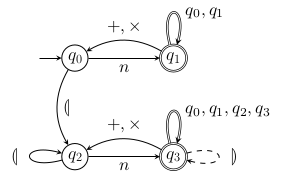
\includegraphics[scale=0.8]{sections/bsp_opa}
\caption{Beispiel OPA}
\label{bsp_opa}
\end{figure}
\begin{table}
\begin{tabular}{|l | c | r |}
\hline
Stack & Zustand & Eingabe \\
\hline \hline
$\bot$ & $q_0$ & $n \times (n+n) + n \#$ \\ \hline
$\bot \left[n, q_0 \right]$ & $q_1$ & $\times  (n+n) + n \#$\\ \hline
$\bot $ & $q_1$ & $\times (n+n) \times n \#$ \\ \hline
$\bot \left[\times, q_1 \right] $ & $q_0$ & $ (n+n) \times n \#$ \\ \hline
$\bot \left[\times, q_1 \right] \left[(, q_0 \right] $ & $q_2$ & $ n+n) + n \#$ \\ \hline
$\bot \left[\times, q_1 \right] \left[(, q_0 \right]\left[n, q_2 \right] $ & $q_3$ & $ +n) +n \#$ \\ \hline
$\bot \left[\times, q_1 \right] \left[(, q_0 \right] $ & $q_3$ & $ +n) + n \#$ \\ \hline
$\bot \left[\times, q_1 \right] \left[(, q_0 \right]\left[+, q_3 \right] $ & $q_2$ & $ n) + n \#$ \\ \hline
$\bot \left[\times, q_1 \right] \left[(, q_0 \right]\left[+, q_3 \right]\left[n, q_2 \right] $ & $q_3$ & $ ) + n \#$ \\ \hline
$\bot \left[\times, q_1 \right] \left[(, q_0 \right]\left[+, q_3 \right] $ & $q_3$ & $ ) +n \#$ \\ \hline
$\bot \left[\times, q_1 \right] \left[(, q_0 \right]$ & $q_3$ & $ ) + n \#$ \\ \hline
$\bot \left[\times, q_1 \right] \left[), q_0 \right]$ & $q_3$ & $  + n \#$ \\ \hline
$\bot \left[\times, q_1 \right]$ & $q_3$ & $  + n \#$ \\ \hline
$\bot $ & $q_3$ & $ + n \#$ \\ \hline
$\bot \left[+, q_3 \right]$ & $q_2$ & $ n \#$ \\ \hline
$\bot \left[+, q_3 \right] \left[n, q_2 \right]$ & $q_3$ & $\#$ \\ \hline
$\bot \left[+, q_3 \right]$ & $q_3$ & $\#$ \\ \hline
$\bot $ & $q_3$ & $\#$ \\ \hline
\end{tabular}
\caption{Berechnung der Eingabe durch den Automaten. Jede Zeile steht dabei für eine Konfiguration}
\label{compute}
\end{table}


